\documentclass[11pt]{report}

\usepackage[utf8]{inputenc}
\usepackage[top=2cm, bottom=2cm, left=2cm, right=1.5cm]{geometry}
\usepackage{xspace}
\usepackage[toc,page]{appendix} 
\usepackage[pdftex]{graphicx}
\usepackage{tikz}
\usepackage{tikz-uml}
\usepackage{lscape}
\setlength{\columnseprule}{0.5pt}
 \parskip=10pt
\usepackage{sidecap}
\usepackage{wrapfig}
\usepackage{pgfkeys}
\usepackage{array}
\usepackage{tkz-graph}
\usetikzlibrary{arrows}
\usetikzlibrary{positioning}
\usepackage[francais]{babel}
\usepackage[T1]{fontenc}
\usepackage[bookmarks={true},bookmarksopen={true}]{hyperref}
\usepackage{multicol}
\usepackage{fancyhdr}
\usepackage[babel=true]{csquotes}
\usepackage{url} % Pour écrire des adresses cliquables.
\usepackage{lmodern} % Pour changer le pack de police.
\usepackage{etoolbox}
\usepackage{colortbl}
\usepackage[final]{pdfpages} 
\usepackage{titlesec}
\usepackage{multirow}
\newcommand{\chapterP}{\chapter}
\pagestyle{fancy}
\usepackage{caption}
\usepackage{indentfirst}
\setlength{\parindent}{15pt}


\captionsetup[table]{labelformat=empty}
\renewcommand{\headrulewidth}{1pt}
\fancyhead[L]{La Pastourelle}
\fancyhead[C]{}
\fancyhead[R]{\leftmark}
\renewcommand{\footrulewidth}{1pt}
\fancyfoot[L]{IUT de Rodez}
\fancyfoot[C]{- \thepage -}
\fancyfoot[R]{2015 - 2016}

\usepackage[light,math]{iwona}

\setcounter{secnumdepth}{5}
\renewcommand{\thechapter}{\Alph{chapter}}
\renewcommand{\thesection}{\Alph{chapter}.\Roman{section})}
\renewcommand{\thesubsection}{\Alph{chapter}.\Roman{section}.\arabic{subsection})}
\renewcommand{\thesubsubsection}{\Alph{chapter}.\Roman{section}.\arabic{subsection}.\alph{subsubsection})}
\parskip 5pt

\tikzstyle{line}=[-, thick]


\title{Projet Externe\\La Pastourelle}
\author{DEMERY Cyril\\COSTA Mickael\\MEJANE Thibault\\ZEGHMATI Clément}
\date{2014 - 2015}

\pdfinfo{%
  /Title    (Projet Web - La Pastourelle)
  /Author   (DEMERY Cyril)
  /Creator  (DEMERY Cyril)
  /Producer ()
  /Subject  (La Pastourelle)
  /Keywords ()
}

\begin{document}
\maketitle
\setcounter{tocdepth}{5}
\tableofcontents
\chapter{Plan de Management de Projet}
\section{Introduction}
L'assocation La Pastourelle est une assocation de danses folkloriques 
aveyronnaises. Ce site est destiné aux membres de l'assocation mais aussi aux 
visiteurs externes qui souhaitent suivre les actualités concernant les 
évènements à venir. Il sera donc régulièrement mis à jour par les ayants 
droits de l'assocation. Par conséquent, il faudra que le site soit à la fois 
agréable pour les visiteurs, mais aussi pour toutes les personnes qui 
s'occupent de la mise en forme du contenu.\\

\par Ce dossier est le Plan de Management de Projet, c'est lui qui regroupera 
tous les choix stratégiques sur la manière dont le projet sera conduit : 
l'organisation de l'équipe, la gestion des tâches ainsi que le cahier des 
charges, après une analyse approfondie des besoins du client.

\section{Présentation}
\subsection{Les acteurs}
Ce projet consistera à dialoguer avec une association, et plus particulièment 
avec les personnes suivantes : 
\begin{itemize}
    \item Mr Pagès, secrétaire adjoint de l'assocation\\
\end{itemize}

\par A l'IUT, nos interlocuteurs sont Mr. Belières qui s'occupe de superviser 
l'avancement du projet et de nous aider dans nos éventuels choix techniques, 
ainsi que Mr. Rous qui est chargé du suivi de la gestion de projet.   \\

\par Concernant notre équipe, elle est formé de quatre étudiants de deuxième 
année informatique : 
\begin{itemize}
    \item Mickael Costa
    \item Cyril Démery
    \item Thibault Méjane
    \item Clément Zeghmati
\end{itemize}


\subsection{Enjeux et bénéfices}
Ce projet possède de multiple enjeux. Tout d'abord, le fait de travailler pour 
une association nous impose de fournir un résultat afin de représenter au mieux 
le travail de l'IUT et le sérieux de ces étudiants. Ensuite, travailler pour 
un acteur extérieur, non-scolaire et non-informaticien, est un challenge car il 
faudra utiliser des supports de communication adaptés afin de se faire 
comprendre. \\

\par Concernant l'aspect technique, ce projet ne peut être que bénéfique car il 
va nous apprendre à travailler sur un existant déjà bien établit. Ainsi, il va 
falloir se plonger dans un code qui nous est étranger. Aussi, développer une 
application Web, en l'occurence un site internet, est un plus car c'est une 
domaine en pleine expansion actuellement.\\

\par Enfin, nous pouvons dire que cette expérience sera facilement visible par 
des personnes extérieurs et pourra ainsi nous aider dans la recherche d'un 
emploi.
\subsection{Cahier des charges}
L'équipe projet s'engage à réaliser les taches suivantes :
\subsubsection*{Tâches prioritaires}
Elles sont obligatoires et sont la cause de la rénovation du site, elles doivent être menées à terme en priorité. 

Correction des erreurs graves liées à l'administration :
\begin{itemize}
\item Membre qui ne bascule pas dans l'annuaire après sa validation par un
administrateur
\item Problème de masque de saisie qui empêche de voir l'intégralité du contenu
à modifier 
\item Problème de saisie de la phrase du jour qui ne fonctionne pas en saisie
directe, mais seulement via un copié/collé depuis Word
\item Erreur de caractère dans le planning : impossible de supprimer ou de
modifier un événement contenant un caractère invalide
\end{itemize}

\subsubsection*{Tâches importantes}
Ces tâches seront réalisées dans un second temps et s'il est possible de les effectuer sans trop toucher à la structure du site.
\begin{itemize}
 \item Version multilingue du site : il faut, en plus de l'espagnol, donner la
possibilité d'ajouter du texte en anglais et en occitan 
 \item Ajout de vidéos : donner la possibilité d'intégrer des liens youtube
 \item Dimensionnement automatique des photos : réduire automatiquement la
taille des images, soit à une taille saisie, soit à une taille par défaut 
 \item Changer l'ordre d'affichage des revues
 \item Revoir la carte du monde : corriger le problème de doublon et de
placement du drapeau, ou intégrer un nouveau système de localisation d’évènements
 \item Changement du formulaire de la page des actualités : il faudrait unifier
 les champs afin de ne pas avoir à saisir trop d'informations inutiles
 \item Enlever la mention \og pièce jouée \fg automatique pour la partie théâtre
 qui s'intègre automatiquement si l'on saisit quelque chose
\end{itemize}


\subsubsection*{Tâches secondaires}
Ces éléments sont facultatifs et seront réalisés en fonction de nos disponibilités et du temps restant.
\begin{itemize}
\item Changer la couleur de fond : mettre des couleurs plus modernes
\item Changer les icônes : là aussi, intégrer des éléments plus agréables à
regarder
\item Inclure un responsive design afin de faciliter la navigation depuis
différents supports
\item Repenser le bon de commande afin de le rendre plus attractif
\item Ergonomie et présentation (liens, boutons de connexion, etc, style de
formulaire) afin de faciliter la navigation et l'accès au contenu
\item Changer les photos de la boutique avec des photos plus récentes
\item Inclure un captcha pour éviter des attaques de robots qui ont déjà eu lieu
dans le passé
\end{itemize}

\subsection{Charte du projet}
Le but de ce projet est de pouvoir fournir un site fonctionnel à la MOA, 
correspondant aux exigences initiales en ce qui concerne la mise à jour des 
informations ou bien encore le multilangage, tout en fournissant une 
ergonomie facilitant la visite de personnes externes.\\

\par Pour apprécier ce projet, le client pourra s'appuyer sur les éléments 
suivants : 
\begin{itemize}
    \item Les livrables fournis sont en adéquation avec le cahier des charges
    \item Les engagements initiaux en ce qui concerne la documentation ont été 
tenus
    \item Les livrables exigés ont tous été fournis\\
\end{itemize}

\par L'objectif de ce projet est d'introduire un mode de formation, voire 
d'auto-formation, proche de celui que l'on retrouve en entreprise. C'est pour 
cela qu'il est nécessaire de travailler de façon méthodique et rigoureuse. 
Ainsi, le chef de projet sera chargé de veiller au bon respect des points 
précédents, ainsi qu'à celui des échéances, devra coordonner les différents 
acteurs et sera l'interlocuteur entre le groupe et les acteurs externes.\\

\par En plus du chef de projet, nous nous sommes appuyés sur deux autres rôles 
pour coordonner l'équipe : 
\begin{itemize}
    \item Le gestionnaire de configuration qui s'occupe de gérer les différents 
version du site, des versions des logiciels de chacun, de la sauvegarde des 
informations en cas de soucis, et des choix d'outils de travail.
    \item Le secrétaire dont le but est de garder tous les documents relatifs 
au projet à jour, ainsi que de rédiger les comptes rendus de réunion\\
\end{itemize}

\par Concernant les différents livrables à fournir, nous devons rendre : 
	\begin{itemize}
	  \item le site hébergé, testé et fonctionnel
	  \item un manuel d'utilisateur pour l'assocation
	  \item un dossier projet
	  \item un plan projet
	\end{itemize}


\section{Organisation}
\subsection{Grandes étapes}
Ce projet est particulier car il ne dure qu'un semestre, et par conséquent en 
l'ayant commencé mi-octobre et devant le rendre mi-décembre, il ne durera que 
deux mois. \\
\par Nous allons toutefois essayer de le scinder en deux, avec une première 
partie de réponse aux exigences de l'assocation, et une seconde partie basée 
sur des améliorations non-proposées mais envisageable.

\subsubsection*{Première partie}
La première partie sera consacrée à la réponse aux exigences initiale. Pour 
cela, nous avons du prendre un rendez-vous avec le client afin de détailler les 
besoins. \\
Nous avons dû réaliser divers documents afin d'assurer le suivi de projet : 
\begin{itemize}
    \item La liste des tâches
    \item Le Gantt
    \item Les diagrammes de cas d'utilisation et les scénarios associés
    \item La répartition des tâches
    \item Les comptes rendus de réunion \\
\end{itemize}

\subsection{Rôles}
En ce qui concerne la gestion des rôles pour ce projet, nous avons choisit de 
les fixer dès le début et au vu de la durée du projet, de ne pas les modifier, 
ainsi on obtient le tableau suivant :  
\par
\begin{tabular}{ | c | c | }
\hline 
   COSTA Mickael & Pas de rôle  \\ \hline 
   DEMERY Cyril & Chef de Projet / Gestionnaire de configuration \\ \hline 
   MEJANE Thibault & Secrétaire de projet \\ \hline 
   ZEGHMATI Clément & Pas de rôle \\ \hline
 \end{tabular}
\subsection{Méthodes de suivi de projet}
Nous avons décidé de suivre un modèle en V, car le projet est trop court pour 
des itérations de 3 semaines, et ainsi nous pouvons tester les fonctionnalités 
au fûr et à mesure qu'elles sont implantées.
\begin{figure}[htp] \centering{
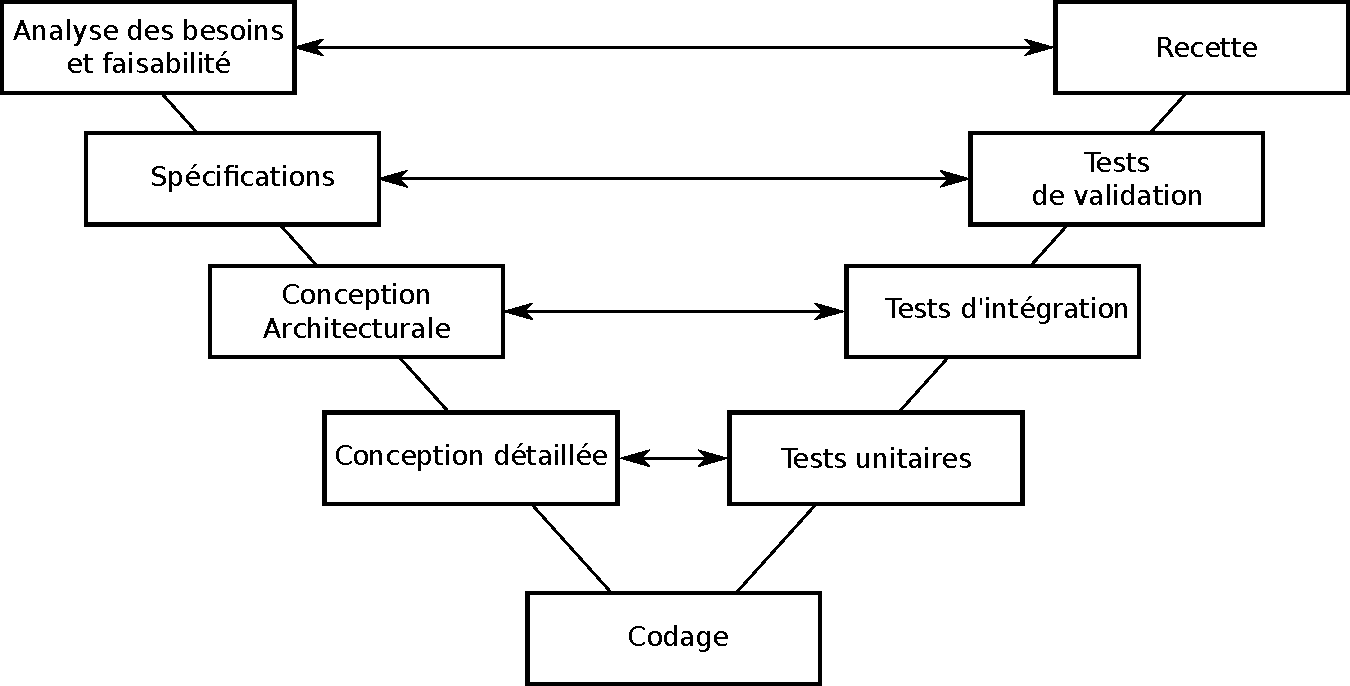
\includegraphics[scale=0.60]{include/cycle_v.pdf}}
\caption{Modèle en V}
\end{figure}

\subsection{Plan de communication}
Durant les périodes scolaires, nous sommes tous présents sur Rodez, mais étant 
donné que pendant les vacances et les week-end nous rentrons dans nos 
départements respectifs, il devient tout de suite plus difficile de communiquer.
C'est pourquoi nous avons décidé d'utiliser Skype combiné à TeamViewer. Ces 
deux outils nous permettent de travailler en binôme quelque soit la distance, 
et ainsi de pouvoir intéragir avec le reste du groupe.\\
\par Toutefois, nous devons nous réunir régulièrement afin de définir la 
stratégie à suivre et de programmer les réunions avec les différents 
intervenants. A ce titre, il serait pertinent de rencontrer la MOA mi-octobre, 
puis début novembre et enfin vers le 20-25 novembre afin de l'informer 
de l'anvancée du projet et d'établir les divers travaux à effectuer.
\newpage

\subsection{Modèles de documents}
\begin{figure}[htp] \centering{
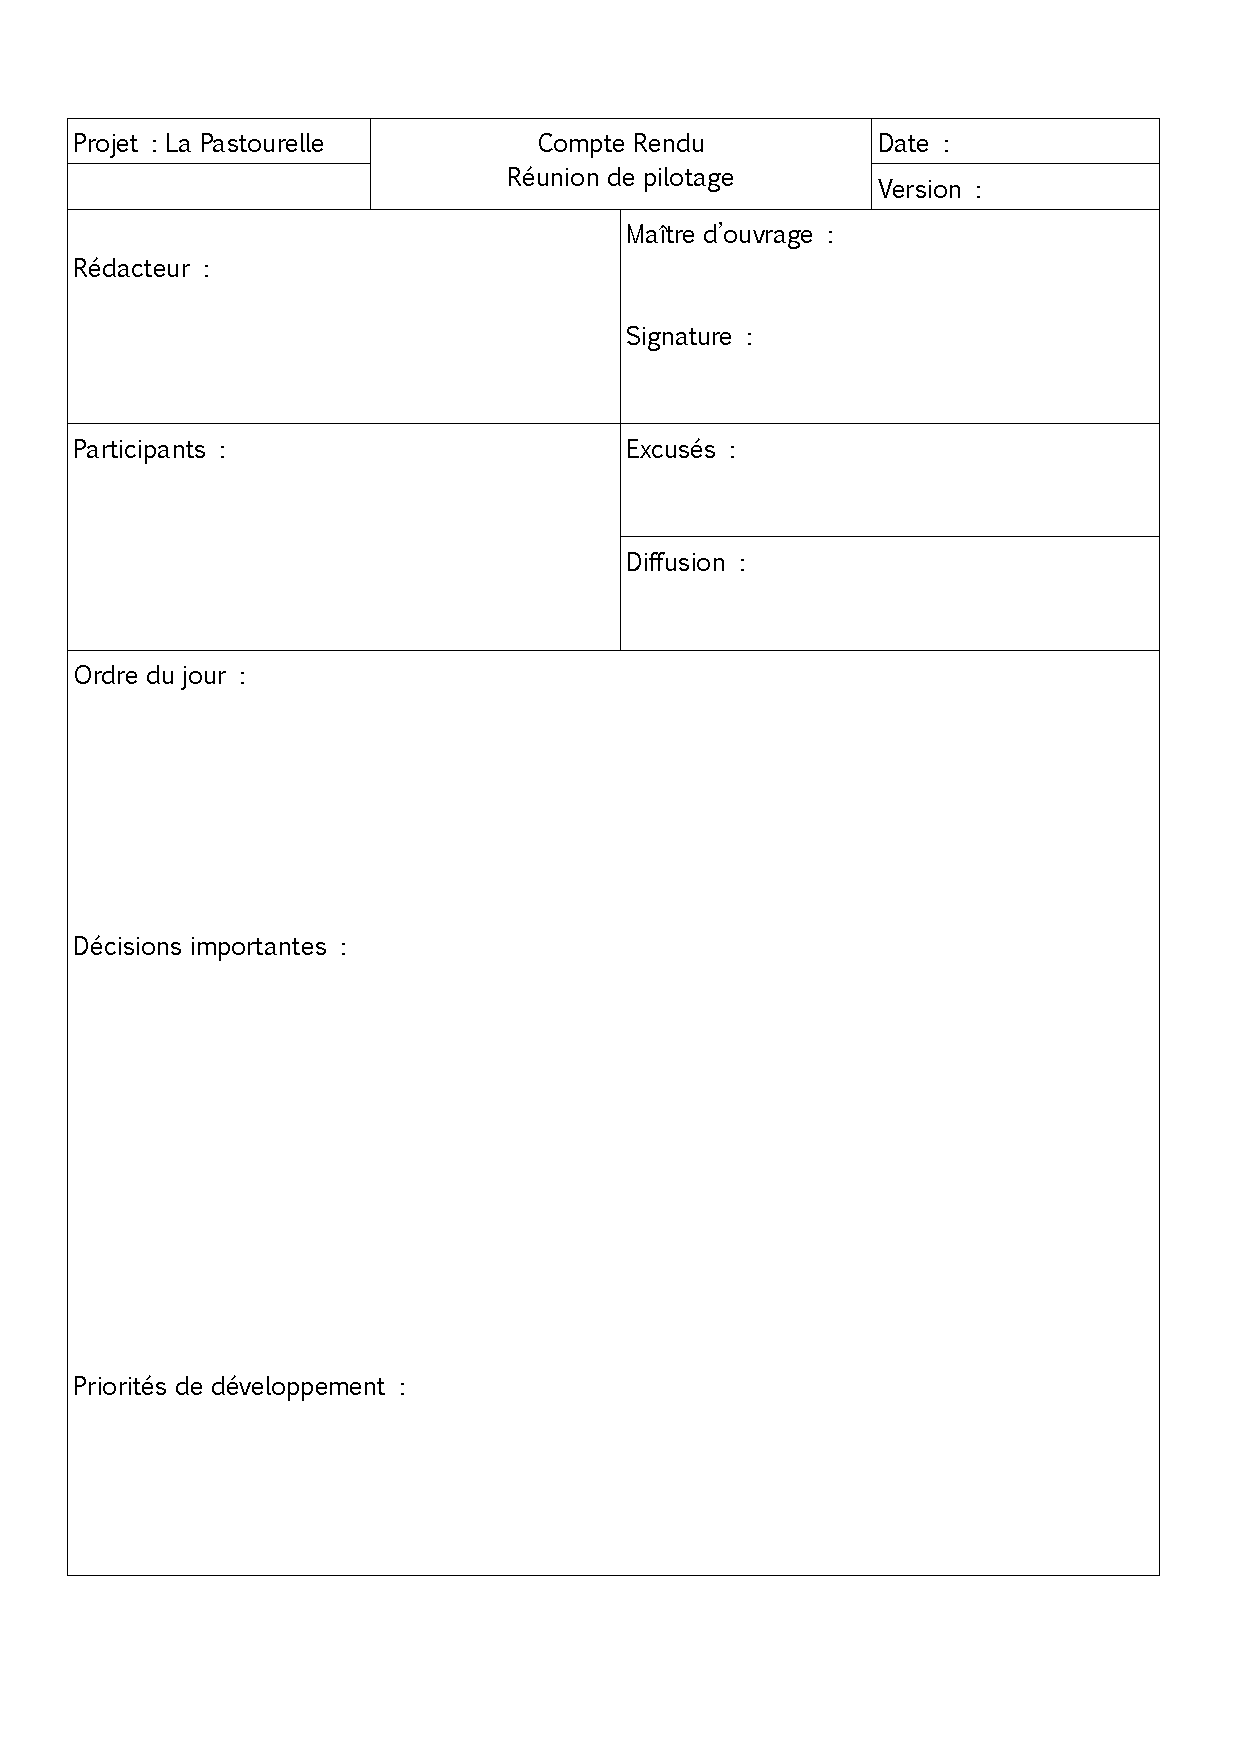
\includepdf[scale=0.80]{include/copil_template.pdf}}
\caption{Modèle de COPIL}
\end{figure}
\newpage
\begin{figure}[htp] \centering{
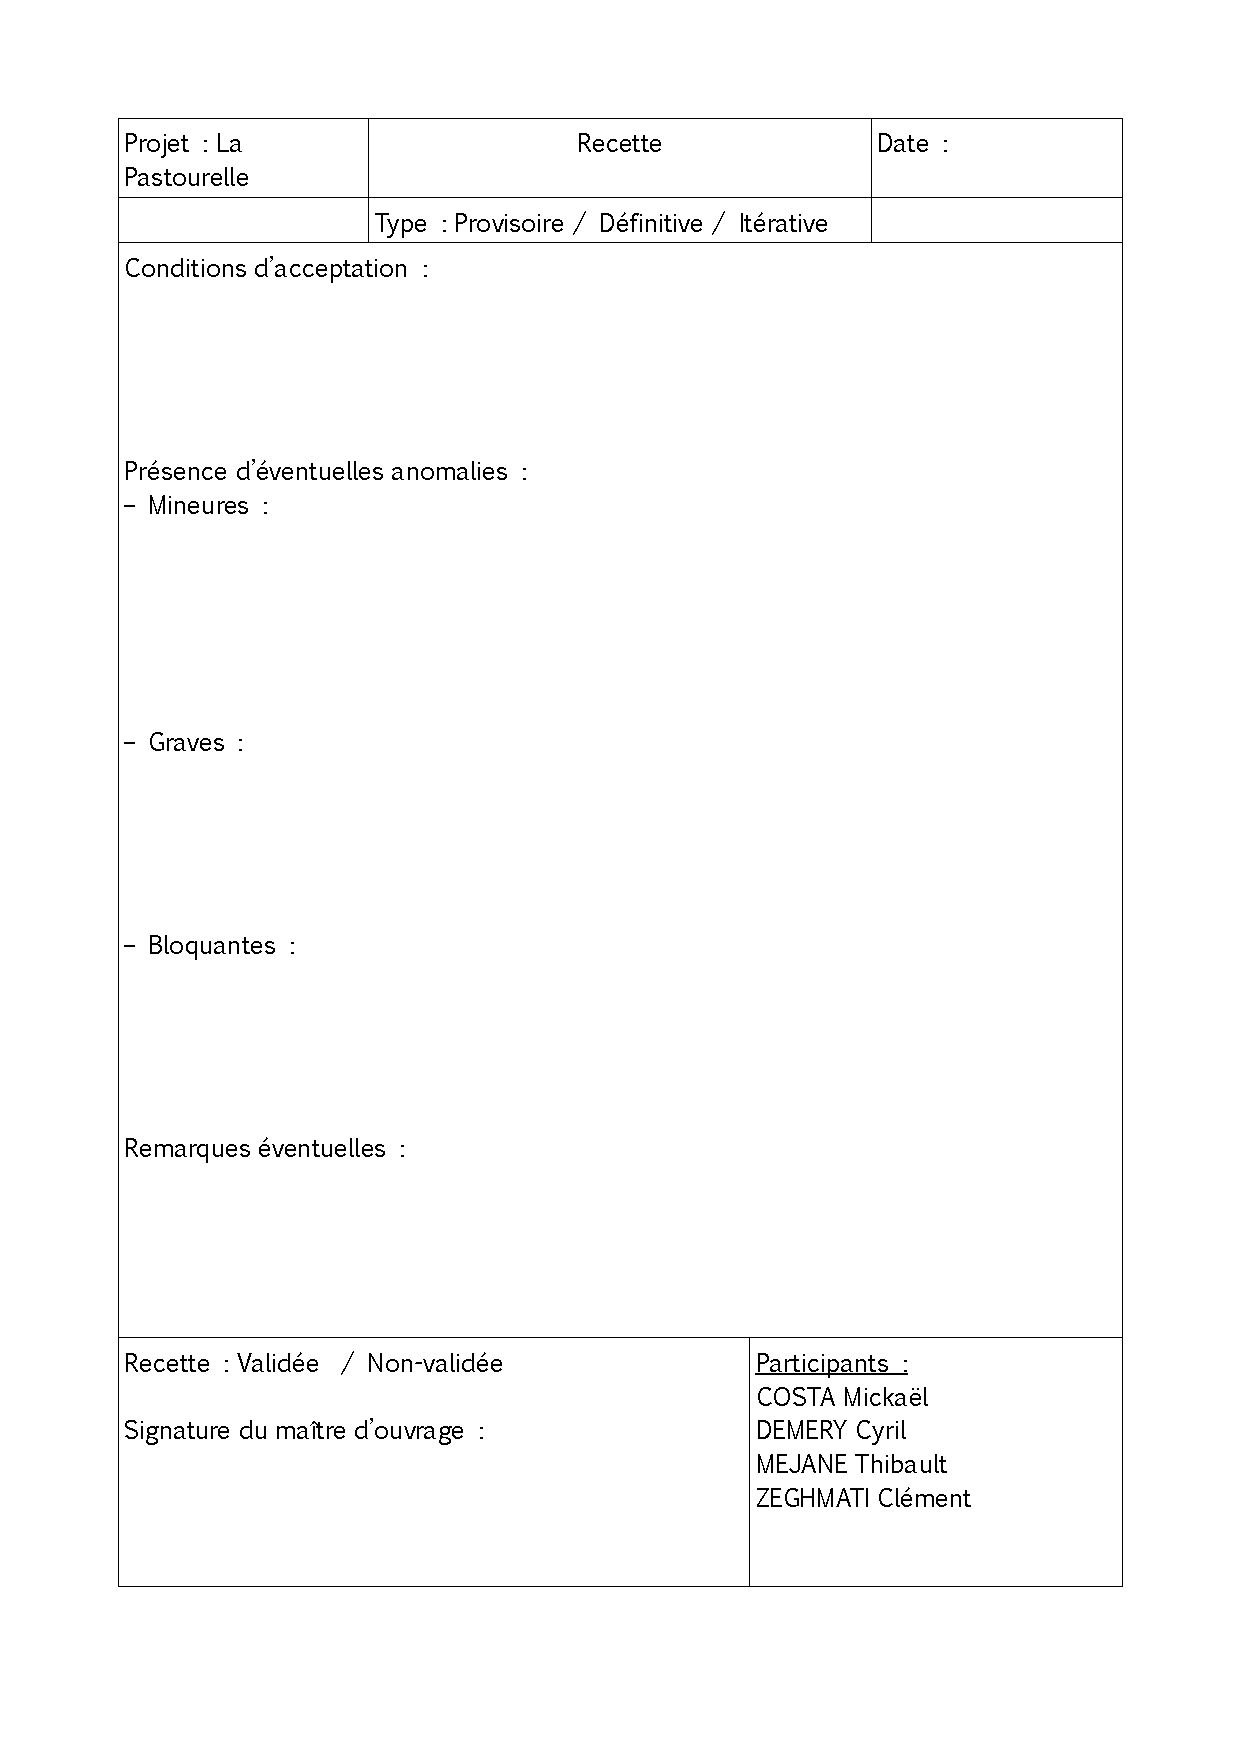
\includepdf[scale=0.80]{include/recette_template.pdf}}
\caption{Modèle de recette}
\end{figure}
\newpage

\subsection{Comité de pilotage}

\subsection{Gestion de la configuration}
Pour ce projet, le gestionnaire de configuration, Cyril, a décidé d'utiliser
les logiciels suivants : \\ 
\par 
\begin{tabular}{ | c | c | c | }
\hline 
   Logiciel & Version & Plugin  \\ \hline 
   LaTeX & 2.22 & tickzuml \\ \hline 
   LibreOffice & 4.2.8 & spellchecker \\ \hline 
   Eclipse PHP & Luna & texclipse, egit, pdf4linux \\ \hline
   PHP & 5.6 & PDO \\ \hline
   Apache & 2 & \\ \hline
   MySQL & 5.6.27 & \\ \hline
   PhpMyAdmin & 4.5 & \\ \hline
 \end{tabular}
 
 \par En ce qui concerne le travail collaboratif, les codes sources seront
 hébergés sur GitHub de manière à pouvoir les manipuler facilement depuis
 n'importe où, et de toujours conserver la dernière version stable. Pour la
 partie gestion de la plannification, nous utilisons Redmine installé en SaaS
 sur OpenShift afin de pouvoir consulter les tâches à effctuer depuis n'importe
 où, ainsi qu'accéder à la dernière version des documents projets, même si le
 rapport est hébergé sur Github.
 \par Les rapports seront rédigés la plupart du temps en LaTeX afin de
 s'affranchir du système d'exploitation, car certains utilisent Linux et
 d'autres Windows. 

\section{Pilotage}
\subsection{Prévision initiale}
Initialement, nous avions prévus de suivre cette plannification, avec la
première partie jusqu'au jalon définie avec un peu de précision, puis la suite
beaucoup moins car nous devions faire le point avec le client pour voir si le
résultat de la première partie lui convenait.
\par
\begin{tabular}{ | c | p{4cm} | c | c | c | c | c | c | c |  }
\hline 
Id & Tâche & Statut & Priorité & Estimée (h) & Début & Fin & Réalisé &
Préd. \\ \hline
24 & Recoder l'administration du multilangue & A réaliser & Moyenne & 3 &
	21/10/15 & 18/11/15 & 0 & \\ \hline
23 & Correction erreurs diverses (planning)
	& A réaliser & Moyenne & 1 & 21/10/15 & 11/11/15 & 0 & \\ \hline
22 & Correction encodage & A réaliser & Urgente & 5 & 21/10/15 & 11/11/15 & 0
	 & \\ \hline
21 & Correction de l'inscription & Terminé & Haute & 3 & 21/10/15 &
	11/11/15 & 0 & \\ \hline
20 & Inclure un captcha & A réaliser & Basse & ? & 13/11/15 &
	09/12/15 & 0 & 5 \\ \hline
19 & Revoir l'ergonomie et la présentation & A réaliser & Basse & ? & 13/11/15
	& 09/12/15 & 0 & 5 \\ \hline
18 & Changer les photos de la boutique & A réaliser & Basse & ? & 13/11/15 &
	09/12/15 & 0 & 5 \\ \hline
17 & Repenser le bon de commande & A réaliser & Basse & ? & 13/11/15 & 09/12/15
	& 0 & 5 \\ \hline
16 & Inclure un responsive design & A réaliser & Basse & ? &
	13/11/15 & 09/12/15 & 0 & 5 \\ \hline
15 & Changer la couleur de fond & A réaliser & Basse & ? & 13/11/15 & 09/12/15
	& 0 & 5  \\ \hline
14 & Correction de l'ajout des pièces de théâtre & A réaliser & Haute & 2 &
	13/11/15 & 09/12/15 & 0 & 5 \\ \hline
13 & Changement du formulaire de la page d'actualité & A réaliser & Haute & 3 &
	21/10/15 & 11/11/15 & 0 & \\ \hline
12 & Revoir la carte du monde & A réaliser & Haute & 3 & 21/10/15 & 11/11/15 & 0
	& \\ \hline
11 & Changer l'ordre d'affichage des revues & A réaliser & Haute & 1 & 21/10/15
	& 11/11/15 & 0 & \\ \hline
10 & Dimensionnement automatique des photos & A réaliser & Haute & 1 & 21/10/15
	& 03/11/15 & 0 & \\ \hline
9 & Ajout de vidéos & A réaliser & Haute & 1 & 21/10/15 & 03/11/15 & 0 & \\
\hline
8 & Changer les icones & A réaliser & Basse & ? & 21/10/15 & 09/12/15 & 0 & \\
\hline
7 & Version multilingue & A réaliser & Haute & 20 & 21/10/15 & 03/11/15 & 0 & \\
\hline
6 & Erreur de validation & A réaliser & Haute & 3 & 21/10/15 & 03/11/15 & 0 & \\
\hline
5 & Fin de correction des réalisation urgentes et importantes & Jalon & Basse &
	/ & 12/12/15 & 12/11/15 & 0 & \\ \hline
4 & Caractères indésirables dans le planning & Terminé & Urgente & 5 & 21/10/15
	& 03/11/15 & 0 & \\ \hline
3 & Saisie de la phrase du jour & A réaliser & Urgente & 2 & 21/10/15 & 03/11/15
	& 0 & \\ \hline
2 & Correction du masque de saisie & A réaliser & Urgente & 3 & 21/10/15 &
	03/11/15 & 0 & \\ \hline
 \end{tabular}
 \begin{landscape}
   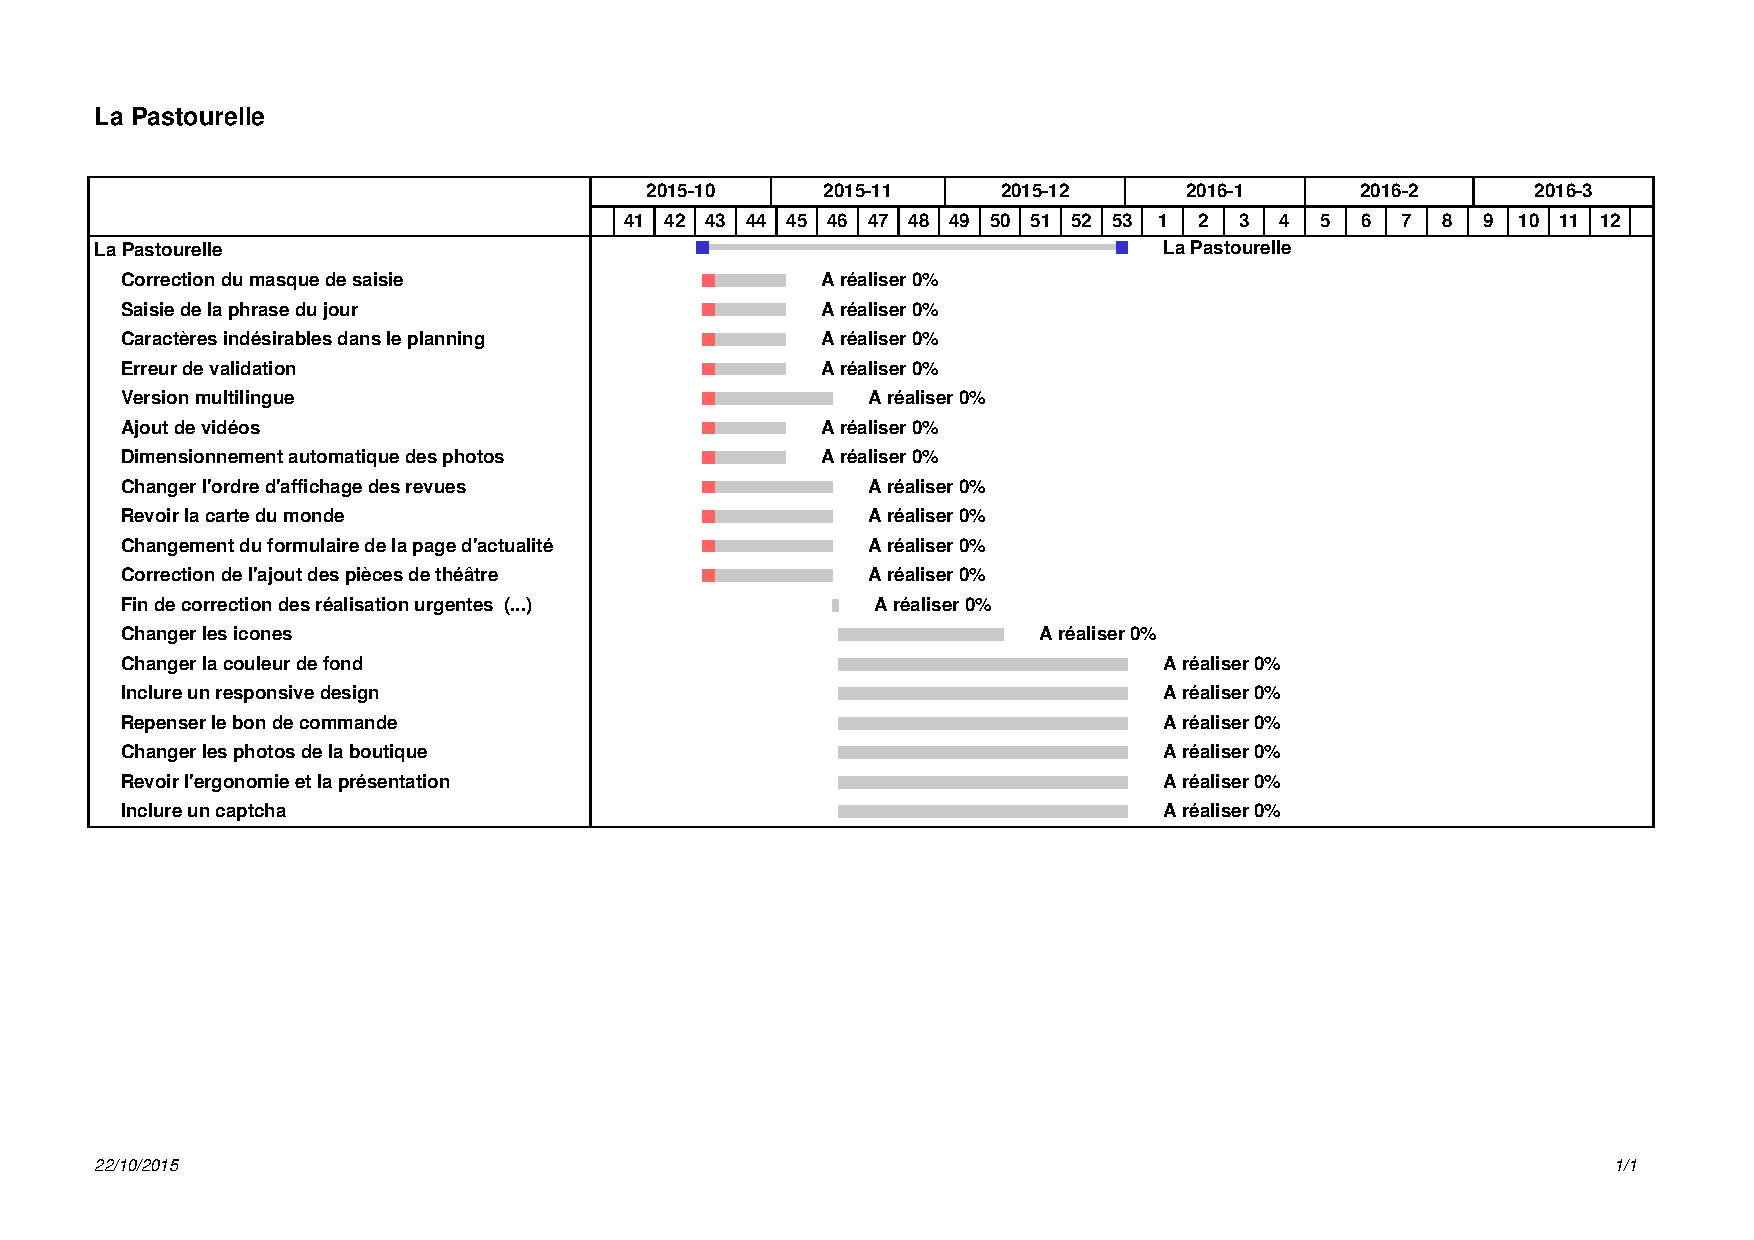
\includepdf{include/gantt22-10.pdf}
\end{landscape}
\clearpage

\subsection{Evolution de la plannification}
Par la suite, la plannification a évolué, ainsi au 3 novembre 2015, soit juste
après les vacances, il se trouve que nous en étions à ce niveau (voire page
suivante). Ici, nous constatons que la plupart des tâches qui étaient à
effectuer pour le retour des vacances n'ont pas été effectuées et, par
conséquent, nous sommes très en retard sur le planning car nous avions prévus
initialement d'effectuer la démonstration avec le client à la mi-novembre.
\par Toutefois, ce retard s'explique par la grande majorité du groupe débute sur
php et n'est pas capable de développer rapidement, ou de s'intégrer sur une
solution déjà développée comme c'est le cas ici. Toutefois, le but de ce projet
est avant tout que tout le monde participe à son développement, donc nous devons
faire avec et les développeurs les plus habiles doivent aider ceux qui sont en
difficultés. 
\par Par conséquent, il est fortement envisageable que nous nous mettions à
travailler en binôme afin de rattraper le temps perdu.
\begin{landscape}
\begin{figure}[t]
    \caption{Avancement du projet au 3 novembre 2015}
   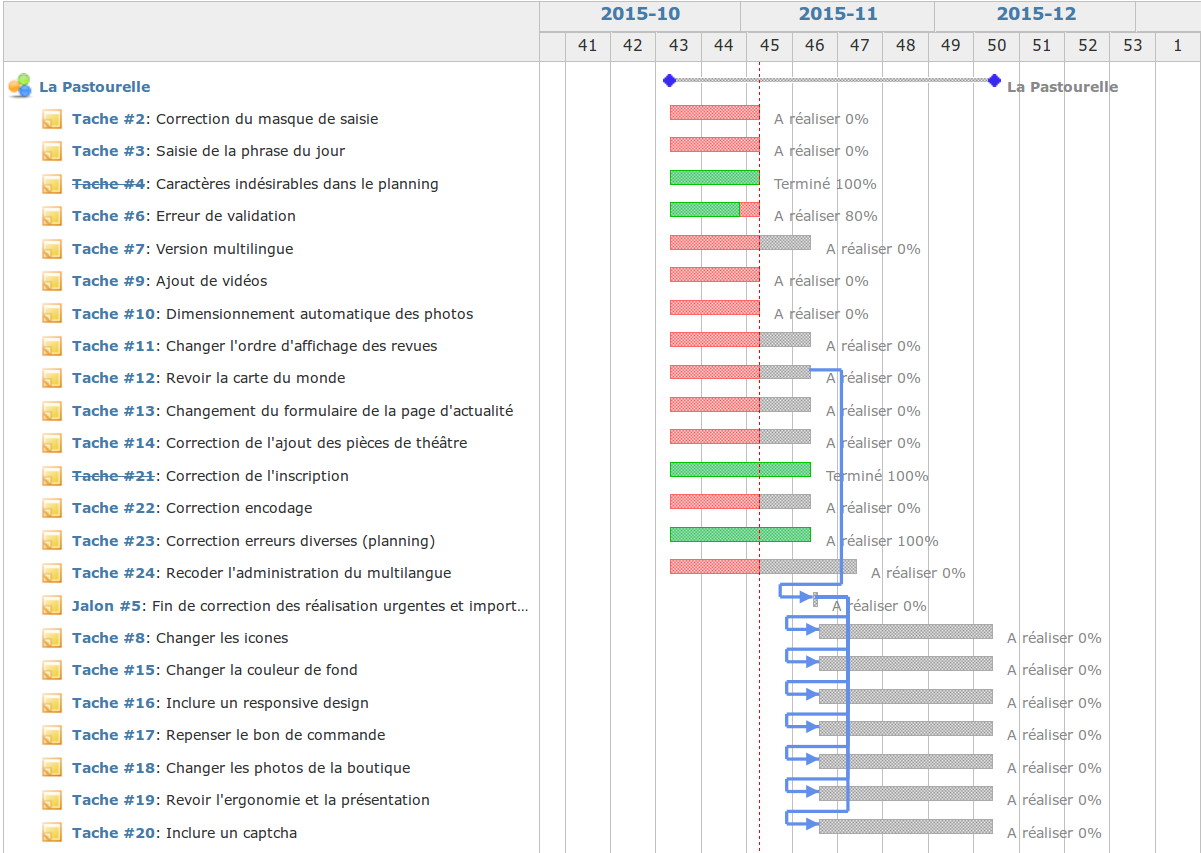
\includegraphics[scale=0.5]{include/gantt3-11.png}
\end{figure}
\end{landscape}

\subsection{Avancement final}

\section{Recettes}

\chapter{Les caractéristiques techniques}
\section{Charte graphique}
// TODO nouvelle charte graphique
\section{Développement}
\subsection{Eléments de sécurisation du site}
Afin d'éviter l'injection SQL, nous avons utilisé PDO, ainsi qu'un contrôle des
formulaires en amont via PHP et Javascript pour limiter au maximum les soucis.
Egalement, nous avons mis à jour le système de protection anti-robot, avec un
système plus facile à utiliser.
\subsection{Codes source}
\section{Base de données}
// TODO mettre le schéma SQL

\chapter{Le déploiement de l'application Web}
\section{Scénario de recettes}
\section{Manuel utilisateur}
\section{Manuel administrateur}
\end{document}